\documentclass[]{friggeri-cv_reccius-experiment}
\usepackage{afterpage}
\usepackage{hyperref}
\usepackage{color}
\usepackage{xcolor}
\PassOptionsToPackage{cmyk}{xcolor}
\usepackage{smartdiagram}
\usepackage{fontspec}
\usepackage{fontawesome}
\usepackage{marvosym}
\usepackage{textcomp}
\usepackage{float} % to position signature
\usepackage{adjustbox}
\usepackage{calc}
\usepackage{enumitem} % to customize indent of bullet points via \itemize
\usepackage{metalogo}
\usepackage{dtklogos}
\usepackage[utf8]{inputenc}	
\usepackage{tikz}
\usetikzlibrary{mindmap,shadows,positioning}
\hypersetup{
    pdftitle={},
    pdfauthor={},
    pdfsubject={},
    pdfkeywords={},
    colorlinks=false,           % no lik border color
    allbordercolors=white       % white border color for all
}
\smartdiagramset{
    bubble center node font = \footnotesize,
    bubble node font = \footnotesize,
    % specifies the minimum size of the bubble center node
    bubble center node size = 0.06cm,
    %  specifies the minimum size of the bubbles
    bubble node size = 0mm,
    % specifies which is the distance among the bubble center node and the other bubbles
    distance center/other bubbles = 0.8cm,
    % sets the distance from the text to the border of the bubble center node
    distance text center bubble = 0.3cm,
    % set center bubble color
    bubble center node color = centergray,
    % define the list of colors usable in the diagram
    set color list = {bubblegray, bubblegray, bubblegray, bubblegray, bubblegray, white, lightgray, lightgray, lightgray, lightgray},
    % sets the opacity at which the bubbles are shown
    bubble fill opacity = 0.7,
    % sets the opacity at which the bubble text is shown
    bubble text opacity = 1,
}

% \addbibresource{bibliography.bib}
\RequirePackage{xcolor}
\definecolor{lightgray}{HTML}{777788}
\definecolor{centergray}{HTML}{F0F6F9}
% you can change ipsgreen to any color you like, but you´ll also have to change it in the reccius-cv-experiment.cls file
\definecolor{ipsgreen}{HTML}{5D78FF}

% NAME AND TAGLINE
\begin{document}
\header{Ilya}{Sevostyanov}
      {Robotics Engineer}
      
\vspace{0.3cm}   
\color{lightgray}\noindent\makebox[\textwidth]{\rule{\paperwidth-0.4cm}{2.5pt}}
% In the aside, each new line forces a line break

%%%%%%%%%%%%%%%%%%%%%%%%%%%%%%%%%%%%%
%%%%%%%%%%%%                 CONTACT                %%%%%%%%%%
%%%%%%%%%%%%%%%%%%%%%%%%%%%%%%%%%%%%%

\begin{info}
    \begin{flushleft}
    {{\hfill{\LARGE \textborn\thinspace\thinspace\verythinspace\hspace{14mm}}\small October 1, 1997}\\
    
    \vspace{0.11cm}
    
    \small \hfill{\Large\faMapMarker\thinspace\thinspace\thinspace\hspace{5mm}} 420500 Innopolis, TR}\
    
    \vspace{0.11cm}
    
    \hfill{\LARGE\Mobilefone\thinspace\hspace{9mm}}{\small +7 (985) 095 27 27}\\

    \vspace{0.11cm}
    
    \hfill{\Large\Letter}\hspace{0.5mm}{\small \faMousePointer  }\hspace{3mm}\href{mailto:sevocrear@gmail.com}{{\small\textbf{sevocrear@}gmail.com}}\\
    
    \end{flushleft}
\end{info}

%%%%%%%%%%%%%%%%%%%%%%%%%%%%%%%%%%%
%%% %%%%%%%%               SIDE BARS               %%%%%%%%%
%%%%%%%%%%%%%%%%%%%%%%%%%%%%%%%%%%%
\begin{aside}
    ~

% PICTURE
\vspace{-3.5cm}
\begin{figure}[ht]
	\hspace{0.3cm}
	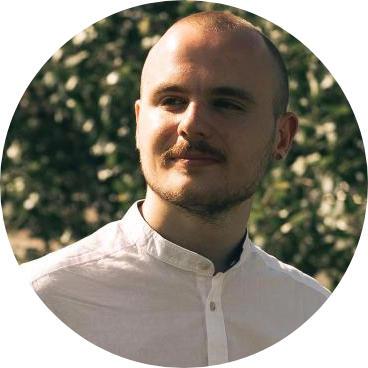
\includegraphics[width=.71\linewidth]{img/Ilya.png}
\end{figure}

% SKILLS
\newcommand{\skillspace}{\vspace*{-0.75mm}}
  \vspace{-2.9mm}
  \section{Skills\thinspace \&\thinspace Strengths}\\
  \vspace{3.5mm}
    
	\textbf{Hard Skills}\\\vspace{0.4mm}
	\begin{itemize}[leftmargin=*, noitemsep]
	\item Python
	\item C++
	\item MATLAB
	\item Robot Operating System (ROS)
	\item Linux
	\item Git
	\item CAD systems
	\item Computer Vision
	\item TeX\\
	\end{itemize}	

  	\skillspace
	\textbf{Soft Skills}\\\vspace{0.4mm}
	\begin{itemize}[leftmargin=*, noitemsep]	
	\item Hard-working
	\item Purposeful
	\item Resolute
	\item Modest
	\item Ultimate team player\\
	\end{itemize}	

  \vspace{-2.6mm}
  \section{Eager to deepen knowledge about:}\\
  	\begin{itemize}[leftmargin=*, noitemsep]
	\vspace{3mm}
	\item Algorithms and databases
	\item Statistics
	\item Machine learning
	\end{itemize}	
  
  \vspace{-2.7mm}
\end{aside}
~
% LANGUAGES
\newcommand{\belowspace}{\vspace*{0.85mm}}
\begin{below1}
  \section{Languages}
    \\\vspace{1.7mm}
    \textbf{Russian}\hfill
    
\includegraphics[scale=0.11]{img/IPSDots.png}
    
\includegraphics[scale=0.11]{img/IPSDots.png}
    
\includegraphics[scale=0.11]{img/IPSDots.png}
    
\includegraphics[scale=0.11]{img/IPSDots.png}
    
\includegraphics[scale=0.11]{img/IPSDots.png}
    
\includegraphics[scale=0.11]{img/IPSDots.png}\\
    \belowspace
    \textbf{English}\hfill
    
\includegraphics[scale=0.11]{img/IPSDots.png}
    
\includegraphics[scale=0.11]{img/IPSDots.png}
    
\includegraphics[scale=0.11]{img/IPSDots.png}
    
\includegraphics[scale=0.11]{img/IPSDots.png}
    
\includegraphics[scale=0.11]{img/WhiteDots.png}
    
\includegraphics[scale=0.11]{img/WhiteDots.png}\\
    \belowspace~  
\end{below1}

% INTERESTS
\begin{below2}
  \section{Interests \& Activities}
    \\\vspace{1.7mm}
    \textbf{Swimming | Gym |\\
    \belowspace 
    Cinema | Driving | \\
    \belowspace
    Travelling}\\
    \belowspace
    
~
\end{below2}
%%%%%%%%%%%%%%%%%%%%%%%%%%%%%%%%%%%
%%% %%%%%%%%             EDUCATION             %%%%%%%%%%
%%%%%%%%%%%%%%%%%%%%%%%%%%%%%%%%%%%
\newcommand{\eduspace}{\vspace*{0.85mm}}
\newcommand{\eduspaceII}{\vspace*{0.8mm}}
\newcommand{\jobspace}{\vspace*{-4.2mm}}
\vspace{-0.5mm}

\section{PROFILE}

Studying for a master's degree in Innopolis University, Russia. Majoring in robotics and mechatronics. Have solid knowledge in the control, kinematics, dynamics of robots. Have experience soldering and assembling circuits, as well as being able to simulate robots.  

Have knowledge in ML: types of training, implementation of various networks and their application, recognition, detection of objects, how to collect, augment datasets and make custom data loaders for them and so on.

Also, worked a lot of time with OpenCV: image processing, video frames, object detections:  the distance to the object calculation using stereo vision; detection of the number plates of the cars using a camera; ping-pong ball tracking, etc.

\section{EDUCATION}
\begin{entrylist}
    
  \entry
    {2019 - 2021\enspace}
    {Computer Science | }{\Large\thinspace\normalsize master degree}
    {\normalsize\textbf{\color{ipsgreen}\faMapMarker\space Innopolis University}}
    {\textbf{Thesis Project:} \\The dynamic walking of quadruped robot
    \eduspace\\}

  \entry
    {2015 - 2019\enspace}
    {Mechatronics and Robotics | } {\Large\thinspace\normalsize bachelor degree}
    {\normalsize\textbf{\color{ipsgreen}\faMapMarker\space Bauman Moscow State Technical University}
    }
    {\textbf{Thesis Project:} \\the development and control of a vertically walking robot with vacuum suction cups \\
    \textbf{Article:} \\\href{https://aip.scitation.org/doi/abs/10.1063/1.5140108}{Simulation in MATLAB of a vertical walking three-link robot \faMousePointer} \\
    \textbf{Achievements:} \\The best student of the robotics department (2018)}
\end{entrylist}
%%%%%%%%%%%%%%%%%%%%%%%%%%%%%%%%%%
%%%%%%%%%%%%       EXPERIENCE       %%%%%%%%%%%%
%%%%%%%%%%%%%%%%%%%%%%%%%%%%%%%%%%
\section{EXPERIENCE}
\begin{entrylist}

  \entry
    {Aug, 2018 - Feb, 2019\enspace}
    {Engineering Assistant | }{\small JBL Robotics}
    {\normalsize\textbf{\color{ipsgreen}\faMapMarker\space Moscow}}
    {\jobspace
    \begin{itemize}[leftmargin=*, itemsep = 0.1em]
    \item Developed ROS nodes to control the robot barista
    \item Designed the stands for cups  and the gripper for the robot itself\\
    \end{itemize}
    }
    
%   \entry
%     {May, 1999\enspace}
%     {Interim Shift Supervisor | }{ \href{https://kingofqueens.fandom.com/de/wiki/International_Parcel_Service}{\small Queens Office \faMousePointer}}
%     {\normalsize\textbf{\color{ipsgreen}\faMapMarker\space International Parcel Service (IPS)}}
%     {\jobspace
%     \begin{itemize}[leftmargin=*, itemsep = 0.1em]
%     \item Brief detour into white collar occupation when the team was in need
%     \item Provided temporary support to the office in the absense of supervisor O´Boyle (personal leave of absense)
%     \item Scheduled routes for drivers
%     \item Managed the budget
%     \item Contributed to the motivation of all drivers and loaders\\
%     \end{itemize}
%     }
    
\end{entrylist}


\section{ACHIEVEMENTS}
\begin{entrylist}

  \entry
    {Oct, 2020 - Nov, 2020\enspace}
    {Computer Vision Specialist | }{ \href{https://aerobot2020.ru/}{\small "Aerobot 2020" Competition \faMousePointer}}
    {\normalsize\textbf{\color{ipsgreen}\space 1st Place}}
    {\jobspace
    \begin{itemize}[leftmargin=*, itemsep = 0.1em]
    \item Developed ROS node in order to get the offset and rotation of the line\\ with respect to the drone camera
    \item Developed ROS node in order to get the position of the landing stage \\ and remember is so drone could return back after finishing the task\\
    \end{itemize}
    }
    
%   \entry
%     {May, 1999\enspace}
%     {Interim Shift Supervisor | }{ \href{https://kingofqueens.fandom.com/de/wiki/International_Parcel_Service}{\small Queens Office \faMousePointer}}
%     {\normalsize\textbf{\color{ipsgreen}\faMapMarker\space International Parcel Service (IPS)}}
%     {\jobspace
%     \begin{itemize}[leftmargin=*, itemsep = 0.1em]
%     \item Brief detour into white collar occupation when the team was in need
%     \item Provided temporary support to the office in the absense of supervisor O´Boyle (personal leave of absense)
%     \item Scheduled routes for drivers
%     \item Managed the budget
%     \item Contributed to the motivation of all drivers and loaders\\
%     \end{itemize}
%     }
    
\end{entrylist}


% % SIGNATURE
% \vspace{-12.5mm}
% \begin{figure}[H]
% \hspace{11cm}
% \includegraphics[scale=0.5]{img/KevinJamesSignature.jpg}
% \end{figure}
% \vspace{-1.05cm}
% \hspace{6.5cm} Queens, NY, May 14th, 2007
\end{document}